
% v2-acmsmall-sample.tex, dated March 6 2012
% This is a sample file for ACM small trim journals
%
% Compilation using 'acmsmall.cls' - version 1.3 (March 2012), Aptara Inc.
% (c) 2010 Association for Computing Machinery (ACM)
%
% Questions/Suggestions/Feedback should be addressed to => "acmtexsupport@aptaracorp.com".
% Users can also go through the FAQs available on the journal's submission webpage.
%
% Steps to compile: latex, bibtex, latex latex
%
% For tracking purposes => this is v1.3 - March 2012
\documentclass[prodmode,acmtecs]{acmsmall} % Aptara syntax
\usepackage[spanish,polish]{babel}
\usepackage[T1]{fontenc}
\usepackage{fancyvrb}
\usepackage{graphicx,hyperref}
\newcommand\cutout[1]{}


\usepackage[table]{xcolor}
\usepackage[utf8]{inputenc}
\usepackage[parfill]{parskip}
\usepackage{tabulary}
\PassOptionsToPackage{hyphens}{url}
\usepackage{hyperref}    
\usepackage[capitalize]{cleveref}


% Metadata Information
% !!! TODO: SET THESE VALUES !!!
\acmVolume{0}
\acmNumber{0}
\acmArticle{CFP}
\acmYear{0}
\acmMonth{0}

\newcounter{colstart}
\setcounter{page}{4}

\RecustomVerbatimCommand{\VerbatimInput}{VerbatimInput}%
{
%fontsize=\footnotesize,
fontfamily=\rmdefault
}


\newcommand{\UnderscoreCommands}{%\do\verbatiminput%
\do\citeNP \do\citeA \do\citeANP \do\citeN \do\shortcite%
\do\shortciteNP \do\shortciteA \do\shortciteANP \do\shortciteN%
\do\citeyear \do\citeyearNP%
}

\usepackage[strings]{underscore}



% Document starts
\begin{document}


\setcounter{colstart}{\thepage}

\acmArticle{CFP}
\title{{\huge\sc SIGLOG Monthly 279}

 November 2026}\author{ELLI ANASTASIADI\affil{Aalborg University, SE}\vspace*{-2.6cm}\begin{flushright}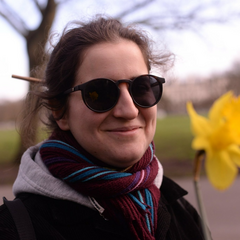
\includegraphics[width=30mm]{elli_anastasiadi.png}\end{flushright}}\begin{abstract}November 2026 edition of SIGLOG Monthly, featuring deadlines, calls and community announcements.
\end{abstract}


\maketitlee

\href{https://lics.siglog.org/newsletters/}{Past Issues}
 - 
\href{https://lics.siglog.org/newsletters/inst.html}{How to submit an announcement}
\section{Table of Contents}\begin{itemize}\item DEADLINES (\cref{deadlines}) 
 
\item SIGLOG MATTERS 
 
\begin{itemize}\item LICS 2027 (\cref{LICS2027})
\end{itemize} 
\item CALLS 
 
\begin{itemize}\item FSCD 2027 (CALL FOR PAPERS) (\cref{FSCD2027})
\item ACM SIGAI Autonomous Agents Research Award (CALL FOR NOMINATIONS) (\cref{ACMSIGAIAutonomousAgentsResearchAward})
\end{itemize} 
\item JOB ANNOUNCEMENTS 
 
\begin{itemize}\item PhD on dynamic logic and planning in Toulouse (\cref{PhDondynamiclogicandplanninginToulouse})
\end{itemize} 
\end{itemize}\section{Deadlines}\label{deadlines}\rowcolors{1}{white}{gray!25}\begin{tabulary}{\linewidth}{LL}FSCD and CADE 2027:  & Dec 04, 2026 (Workshop proposal deadline) \\
ACM SIGAI Autonomous Agents Research Award:  & Dec 05, 2026 (Nomications deadline) \\
LICS 2027:  & Jan 14, 2027 (Titles and short abstracts), Jan 21, 2027 (Full papers) \\
DEON 2027:  & Mar 05, 2027 (Abstract), Mar 12, 2027 (Paper) \\
FSCD 2027:  & Apr 19, 2027 (Abstract), Apr 26, 2027 (Submission), Jun 28, 2027 (Notification) \\
\end{tabulary}
\section{LICS 2027: LOGIC IN COMPUTER SCIENCE }\label{LICS2027}  Montreal, 21–24 June 2027\\ 
  \href{https://lics.siglog.org/lics27/}{https://lics.siglog.org/lics27/}\\ 
CALL FOR PAPERS 

\begin{itemize}\item  IMPORTANT DATES 
 
\rowcolors{1}{white}{gray!25}\begin{tabulary}{\linewidth}{LL}Titles and short abstracts:  & Jan 14, 2027 \\
Full papers:  & Jan 21, 2027 \\
Author response:  & Mar 25, 2027 \\
Notification:  & Apr 15, 2027 \\
\end{tabulary}
 
\item  New for 2027: limits on the number of submissions per author, arXiv posting within a week of the deadline, and single-blind reviewing. Papers are in LIPIcs format, at most 22 pages excluding references. See the website for details: \href{https://lics.siglog.org/lics27/cfp.php}{https://lics.siglog.org/lics27/cfp.php} 
 
\begin{itemize}\item  Invited speakers: Łukasz Kaiser, Joël Ouaknine.
\item  Tutorials: Laura Kovács, Szymon Toruńczyk.
\end{itemize} 
  Program chairs: Pablo Barceló and Alexandra Silva. 
 
\end{itemize}\section{FSCD 2027: International Conference on Formal Structures for Computation and Deduction}\label{FSCD2027}  Radboud University Nijmegen, The Netherlands\\ 
  23-26 August 2027\\ 
  \href{https://fscd-conference.org/2027}{https://fscd-conference.org/2027}\\ 
CALL FOR PAPERS 

\begin{itemize}\item  FSCD (\href{https://fscd-conference.org/}{https://fscd-conference.org/}) covers all aspects of formal structures for computation and deduction, from theoretical foundations to applications. Building on two communities, RTA (Rewriting Techniques and Applications) and TLCA (Typed Lambda Calculi and Applications), FSCD embraces their core topics and broadens their scope to closely related areas in logic, models of computation, semantics and verification in new challenging areas. 
 
\item  IMPORTANT DATES 
 
  All deadlines are midnight anywhere-on-earth (AoE); late submissions will not be considered. 
 
\rowcolors{1}{white}{gray!25}\begin{tabulary}{\linewidth}{LL}Abstract:  & Apr 19, 2027 \\
Submission:  & Apr 26, 2027 \\
Author Response:  & Jun 08, 2027 \\
Notification:  & Jun 28, 2027 \\
Final Version:  & Jul 10, 2027 \\
\end{tabulary}
 
  For a complete list of topics please visit the online CFP. 
 
\item  PUBLICATION 
 
  The proceedings will be published as an electronic volume in the  Leibniz International Proceedings in Informatics (LIPIcs) of Schloss Dagstuhl. All LIPIcs proceedings are open access. 
 
\item  SPECIAL ISSUE 
 
  There will be a special issue of Logical Methods in Computer Science of selected papers. More details will be provided later. 
 
\item  SUBMISSION GUIDELINES  
 
  The submission site is: \href{https://easychair.org/conferences/?conf=fscd2027}{https://easychair.org/conferences/?conf=fscd2027} 
 
  Submissions must be formatted using the LIPIcs style files and submitted via EasyChair. 
 
  Submissions can be made in two categories: 
 
\begin{itemize}\item  Regular research papers are limited to 15 pages, excluding references and appendices. They must present original research which is unpublished and not submitted elsewhere.
\item  System descriptions are limited to 15 pages, excluding references. Shorter papers are welcome and will be given equal consideration. A system description must present new software tools, or significantly new versions of such tools, in which FSCD topics play an important role. An archive of the code with instructions on how to install and run the tool must be submitted. In addition, a webpage where the system can be experimented with should be provided.
\end{itemize} 
  Submissions must be unpublished and not submitted for publication elsewhere. They will be judged on relevance, significance, originality, correctness, and readability. Reviewers may consider material provided in appendices, but submissions must be self-contained within the page limit. If software or data is relevant to a paper, a link that provides access to the software/data must be provided to enable reproduction of results. 
 
  One author of each accepted paper is expected to register and present the work in person at the conference. In case this is not possible, online presentation will be arranged, but in-person registration will still be required. 
 
\item  BEST PAPER AWARD BY JUNIOR RESEARCHERS 
 
  The programme committee will select a paper in which at least one author is a junior researcher, i.e. either a student or someone whose PhD award date is less than three years from the first day of the meeting. When submitting the paper, other authors should declare to the PC Chair that at least 50% of the contribution is made by the junior researcher(s). 
 
\item  CONTACT 
 
  All questions about submissions should be emailed to: 
 
\begin{itemize}\item  Daniele Nantes-Sobrinho        (dnantes 'at' unb.br)
\item  Mariangiola Dezani-Ciancaglini (dezani 'at' di.unito.it)
\end{itemize} 
\end{itemize}\section{PhD on dynamic logic and planning in Toulouse}\label{PhDondynamiclogicandplanninginToulouse}JOB ANNOUNCEMENT 

\begin{itemize}\item  We welcome applications for a 3 years PhD scholarship on dynamic logic and planning, to be supervised by Philippe Balbiani and Andreas Herzig.  
 
  More details can be found here: \href{https://www.irit.fr/~Andreas.Herzig/Phd_BalbianiHerzig.pdf}{https://www.irit.fr/~Andreas.Herzig/Phd\_BalbianiHerzig.pdf}. Interested students should email a CV, transcripts of bachelor and master degree, and a motivation statement to balbiani@irit.fr, herzig@irit.fr. 
 
\begin{itemize}\item  \href{https://www.irit.fr/~Philippe.Balbiani}{https://www.irit.fr/~Philippe.Balbiani}
\item  \href{https://www.irit.fr/~Andreas.Herzig}{https://www.irit.fr/~Andreas.Herzig}
\end{itemize} 
\end{itemize}\section{ACM SIGAI Autonomous Agents Research Award}\label{ACMSIGAIAutonomousAgentsResearchAward}CALL FOR NOMINATIONS 

  Nominations are solicited for the 2027 ACM SIGAI Autonomous Agents Research Award. This award is made for excellence in research in the area of autonomous agents. It is intended to recognize researchers in autonomous agents whose current work is an important influence on the field. The award is an official ACM award, funded by an endowment created by ACM SIGAI from the proceeds of previous Autonomous Agents conferences. The recipient of the award will receive a monetary prize and a certificate, and will be invited to present a plenary talk at the AAMAS 2027 conference.\\ 
\begin{itemize}\item  How to Nominate 
 
  Anyone can make a nomination, but you may not nominate yourself. Nominations should be made by filling out the below google form and should consist of a short (< 1 page) statement that emphasizes not only the research contributions that the individual has made that merit the award but also how the individual’s current work is an important influence on the field. 
 
\item  NOTE: a candidate can only be considered for the award if they are explicitly nominated. If you believe that someone deserves the award, then NOMINATE THEM -- don't assume that somebody else will!  
 
  Nomination Link: \href{https://forms.gle/NGC1tC2nqUWpanMB6}{https://forms.gle/NGC1tC2nqUWpanMB6} 
 
\item  IMPORTANT DATES 
 
\rowcolors{1}{white}{gray!25}\begin{tabulary}{\linewidth}{LL}Nomications deadline:  & Dec 05, 2026 \\
Announcement of winner:  & Feb 01, 2027 \\
AAMAS Conference:  & 3-7 May, 2027 \\
\end{tabulary}
 
\item  For any questions, please contact Sven Koenig (Award Chair, svenk@uci.edu) or Louise Dennis (SIGAI Vice Chair, louise.dennis@manchester.ac.uk). 
 
\end{itemize}


\bigskip Links: \href{http://siglog.org/}{SIGLOG website}, \href{https://lics.siglog.org}{LICS website}, \href{https://lics.siglog.org/newsletters/}{SIGLOG Monthly}\end{document}